\section{EXPERIMENTAL RESULTS}\label{sec:4experiment}
In this section, we detail the evaluation results for our system.

\subsection{Evaluation Results}
We focus on the detection accuracy about five events, that are body posture, the body rollover, the hand position, the micro body movement and the acoustic events.
%, the classification of micro body movement

\subsubsection{Performance of body posture classification}\label{subsub:bodyposture}
We test the overall classification performance of different body postures. The groundtruth of body postures are recorded by the cameras. We use a  cross-validation approach by training the classifier with the data of one user in turn and testing the rest fourteen users. The averaged accuracy for 15 cases are the final performance, as shown in Fig. \ref{fig:posture_zhu}. We observe that the posture detection accuracy is consistently high across all users, and it does not show major variations across users. This good performance benifits from the distinct characteristics of arm position under different sleeping postures.

\begin{figure}[!t]
 \centering
 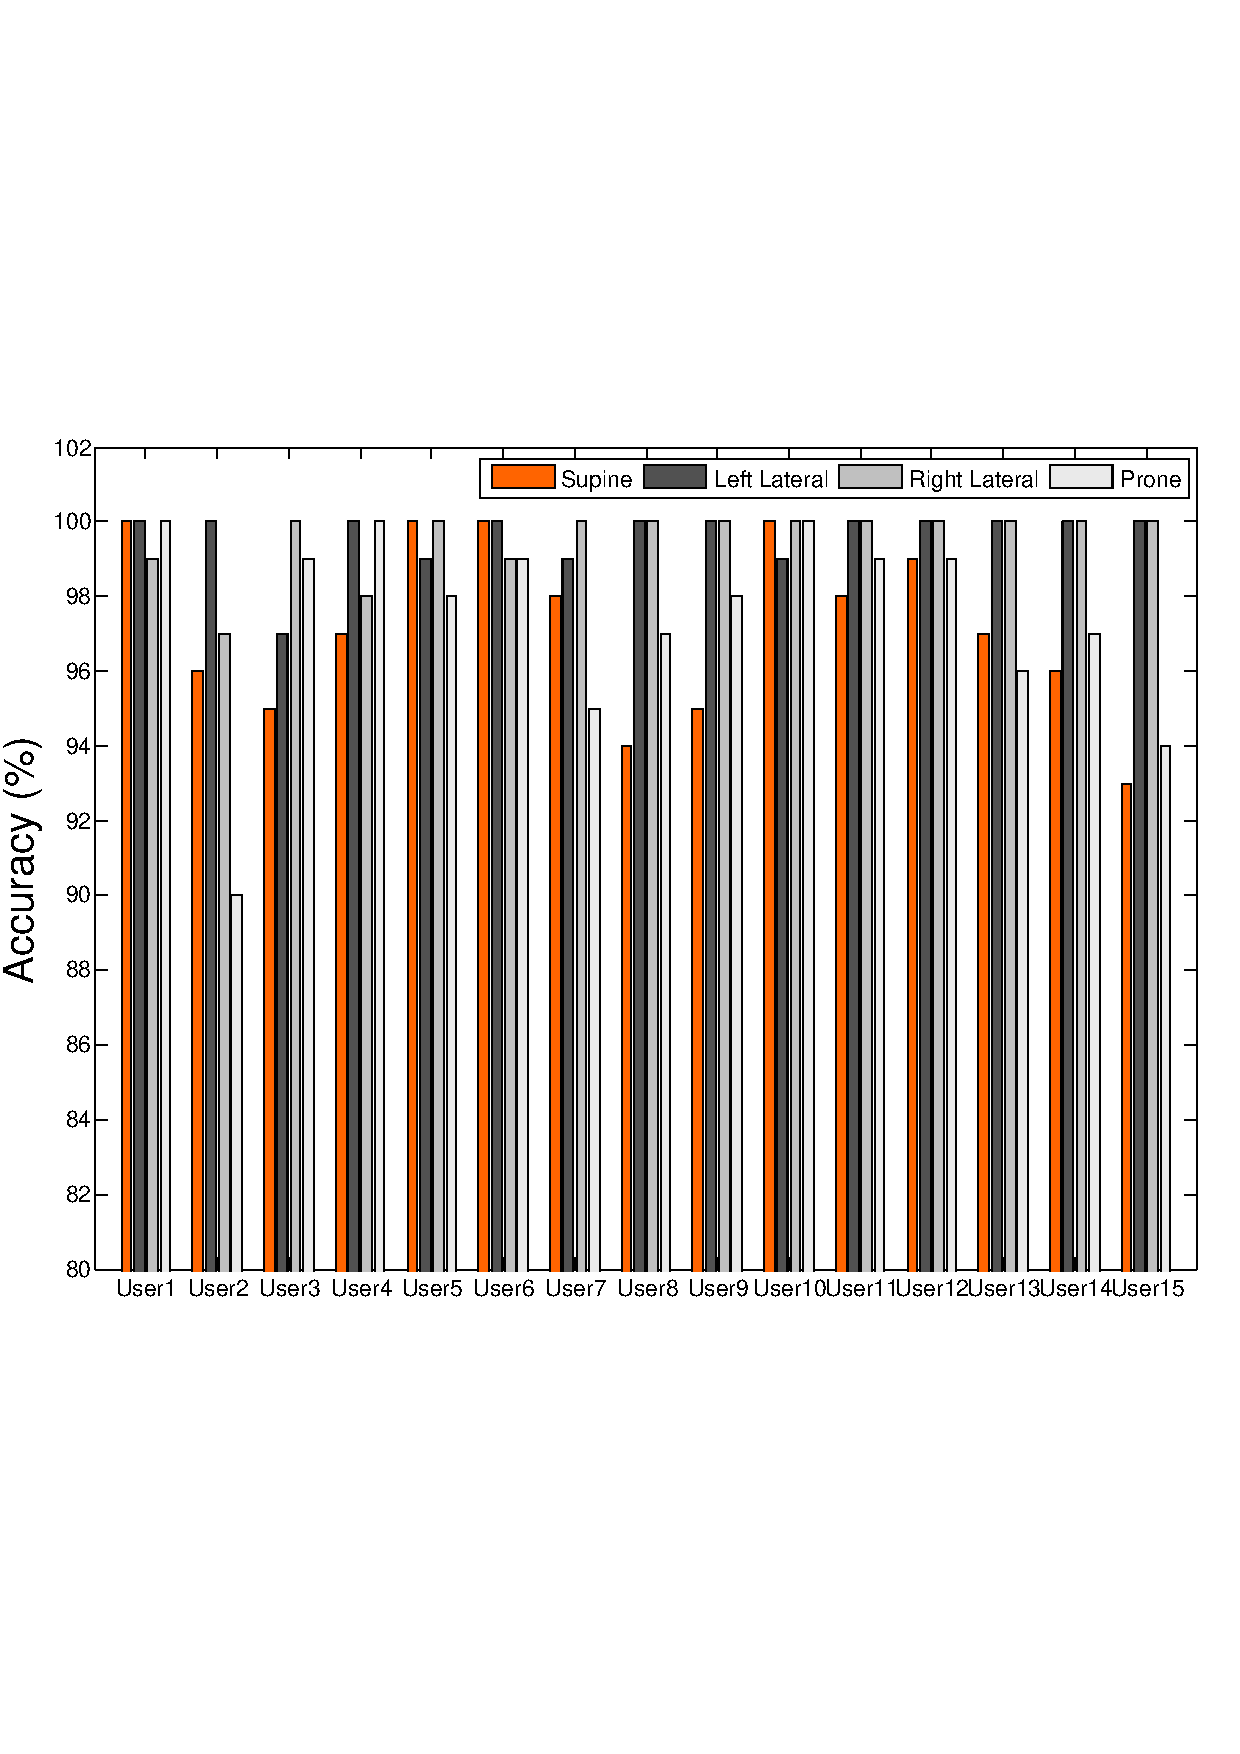
\includegraphics[width=0.52\linewidth]{Figures/posture_zhu.pdf}
 \caption{Detection accuracy of body postures.}\label{fig:posture_zhu}
 \end{figure}

\begin{table}[!thbp]
	\tabcolsep1pt
	\centering  % ������
	%\renewcommand\arraystretch{0.277}
	%\caption{The confusion matrix of body posture classification.}\label{tab:posture}
	%\noindent\makebox{%
	%\begin{tabular}{1\textwidth}{ c | c | c | c | c | c | c}
	\renewcommand\arraystretch{0.3}
	\caption{The confusion matrix of body posture classification.}\label{tab:posture}
	\begin{tabular}{c| c | c | c | c | c | c}
		\cline{1-7}
		&\multicolumn{1}{ c|}{ }
		& \multicolumn{4}{ c|}{ }\\
		\multirow{2}*{}
		&\multicolumn{1}{c|}{\multirow{2}*{{Result}}}
		&\multicolumn{4}{c|}{{Prediction}}
		& \multirow{4}*{{Recall}} \\
		%&\multicolumn{5}{ c |}{\textbf{\small Prediction}} \\
		% & \multicolumn{5}{ c |}{ } \\
		\cline{3-6}
		& & & & & \\
		\multicolumn{1}{c|}{{}}
		&  \multicolumn{1}{c|}{{}}
		&  \multicolumn{1}{c|}{{Supine}}
		&  \multicolumn{1}{c|}{{Left Lateral}}
		&  \multicolumn{1}{c|}{{Right Lateral}}
		&  \multicolumn{1}{c|}{{Prone}}   \\
		& & & & & \\
		\cline{1-7}
		& & & & & \\
		\multirow{5}{*}{\begin{sideways}{{Groundtruth}}\end{sideways}}
		&   {Supine}   & {\bf{{1182}}}    &   $25$      &   $4$      &   $9$    &   {96.7\%}\\
		& & & & & \\
		\cline{2-7}
		& & & & & \\
		&   {Left Lateral}   &   $6$      &   {\bf{{1292}}}     &   $0$      &   $0$   &   {99.5\%} \\
		& & & & & \\
		\cline{2-7}
		& & & & & \\
		&   {Right Lateral}   &   $7$      &   $0$      &  {\bf{{1275}}}      &   $12$  &   {98.5\%}  \\
		& & & & & \\
		\cline{2-7}
		& & & & & \\
		&   {Prone}   &   $19$      &   $2$      &   $3$      &   {\bf{{567}}}   &   {95.9\%} \\
		& & & & & \\
		\cline{1-7}
		& & & & & \\
		&   {Precision}    &   {97.3 \%}   &   {98.0\%}   &   {99.5\%}   &   {96.4\%}    \\
		& & & & & \\
		\cline{1-7}
	\end{tabular}
\end{table}

To have a deep evaluation about the sleep posture detection, we randomly choose one user to train the classifier. Then we calculate the detection precision and recall across postures. The result is shown in Table \ref{tab:posture}. The values in blocks are the corresponding numbers of four sleep postures from 14 test users. Due to that the angle features of acceleration are similar between the suspine posture with hand putting on the head and the left-lateral posture, a small amount of the supine postures are classified as left lateral.  The total amount of the prone posture is less than the number of other postures. It suggests that most people are not accustomed to sleep in the prone posture, because it is neither healthy nor comfortable. In coclude, Table \ref{tab:posture} shows the outstanding detection performance.



\subsubsection{Performance of body rollover counting}
To verify the efficiency of body rollover detection algorithm, we compare each user's  body rollover number detected by {\systemname} with the groundtruth recorded by camera. The performance is showed in Table \ref{tab:rollver}. We can see that User 3, User 4 and User 13 has an unusually high number. For User 3 and User 4, they have difficulty in falling asleep due to the sleep disorder.  User 13 needs to rollover frequently because of  his loundly snoring. For all the 15 users, the detection accuracies are all very high, and the least one is still 87\%. Thus {\systemname} can accurately distinguish the large hand movement from the body rollover in bed. What's more, detecting errors in body rollover events will not have a significant impact on our end result, because the division of  sleep stages is a comprehensive consideration of all the detected features in each stage, such as micro body movement and acoustic events.

\begin{table}[!thbp]
  %\centering  % ������
  \tabcolsep 1pt
  %\arrayrulewidth1pt
  \caption{Detection accuracy of body rollover.}\label{tab:rollver}
   \renewcommand\arraystretch{1.3}{\multirowsetup}{\centering}
        \begin{tabular}{cccccccccccccccc}
        \toprule
         \textbf{User}    & 1& 2  & 3& 4& 5& 6& 7& 8& 9& 10& 11& 12& 13& 14& 15\\
        \midrule
         \rowcolor{Gray}      { Groundtruth}  &231&204&442&397&198&101&196&164&193&208&131&205&342&149&156 \\
                 { Accuracy} &91\%& 94\% &88\%&93\%&96\%&94\%&87\%&90\% &93\% &94\% &92\% &94\% &89\% &90\% &95\%\\
        \bottomrule
 \end{tabular}
\end{table}

\subsubsection{Performance of hand position recognition}
To test the recognition performance of different hand positions, {\systemname} uses the cross-validation approach presented in \ref{subsub:bodyposture} with only one user's data at a time to train the classifier and the remaining 14 users' data as the test sets. The classifier for detecting the hand movement trajectory is combined with the detection of periodic signals caused by respiration, then the hand position on the chest (or abdomen or head) can be identified. Fig. \ref{fig:hand_zhu} illustrates the accuracy of hand position across 15 users. As we can see that with just one set of training data, the accuracies for different users are all higher than 87\%. Therefore, our system can achieve a satisfied identification accuracy for different hand positions. Moreover, we find that at least four out of fifteen participants tends to put their hands on their heads when they sleep in the supine posture.  It is a bad habit and suggests the users to remove the 


\begin{figure}
 \centering
 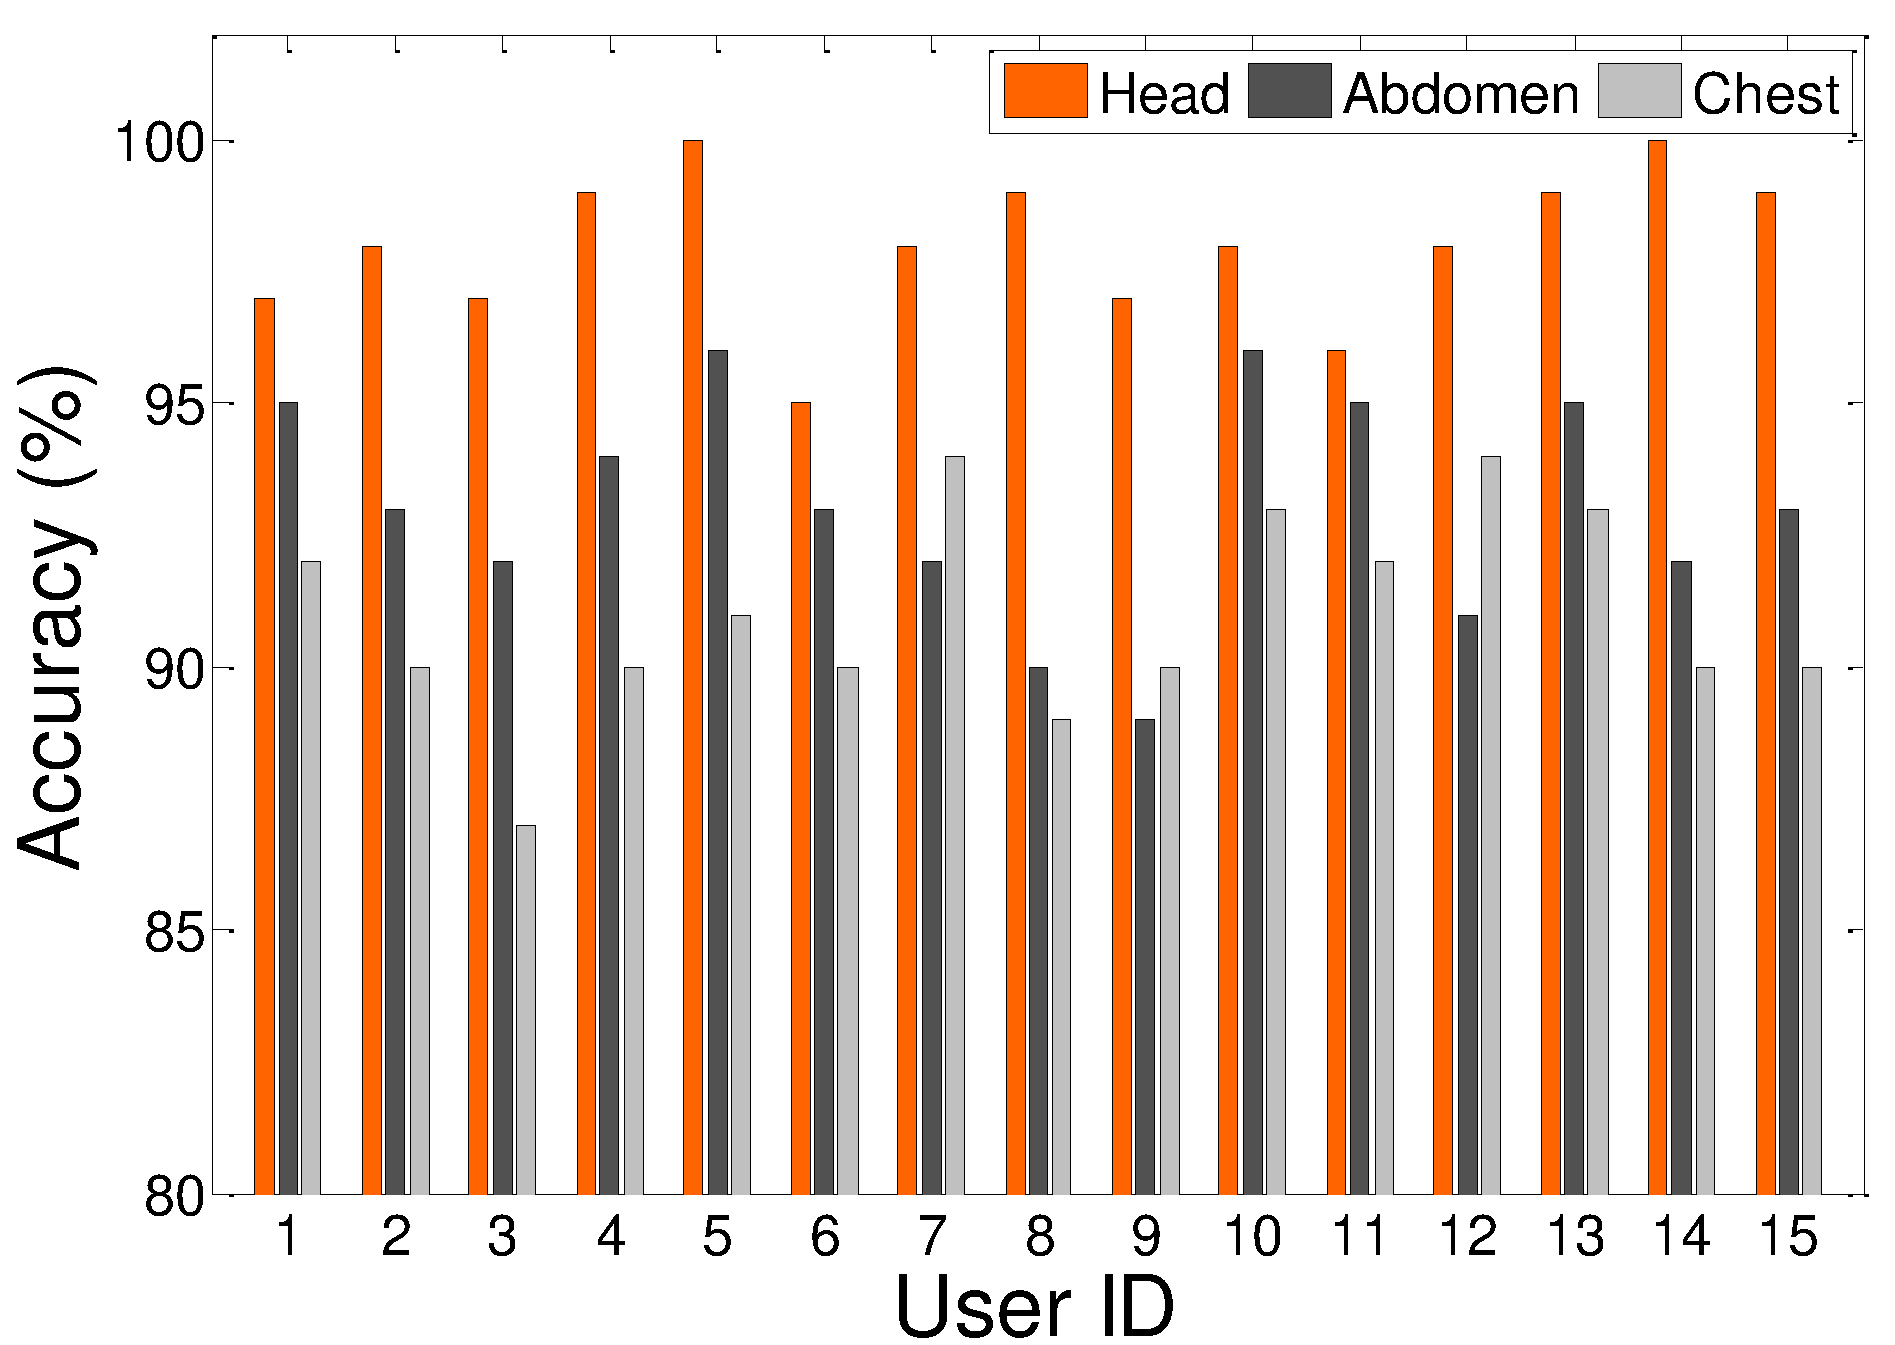
\includegraphics[width=0.52\columnwidth]{Figures/handposition_zhu.pdf}
 \caption{Identification accuracy of hand positions}\label{fig:hand_zhu}
\end{figure}




\subsubsection{Performance of micro body movement detection}
To assess the detection accuracy of micro body movement , we manually label the ground truth  recorded by the camera during sleep, indluding hand moving, arm raising, and body trembling. We also use the accelerometer embedded in the smartphone which placed on the bed to record the occurrence of the micro body movements, so as to avoid missing some movements such as trembling shaded by the coverings (such as quilts). Fig. \ref{fig:micro_movement_zhu} illustrates the detection accuracy across 15 users. It shows that the accuracies for all users are very close, that is, there will be no major changes between users. And from Fig. \ref{fig:micro_combine}, we can see that even though the worst classification result belongs to the hand movement, the average precision and recall rate still exceed 75\%, and the average accuracy of arm raising and body trembling are 93 \%, 84\%, which indicates that the accuracy of the classification is acceptable. And our purpose of detecting micro body movement is to help us detect the sleep stage, so we are more concerned with body trembling and arm raising, and the poor accuracy of hand moving does not have a significant impact on our end result. The reason for the poor performance of hand movement and body trembling classification may be that we have fewer people to refer to when setting the threshold of the peak value. Specifically, we can further consider more different people in different situations, or set their own thresholds for each person by observing or learning each person's sleep data.


\begin{figure}
\setlength{\abovecaptionskip}{0.cm}
\setlength{\belowcaptionskip}{-0.cm}
 \centering
 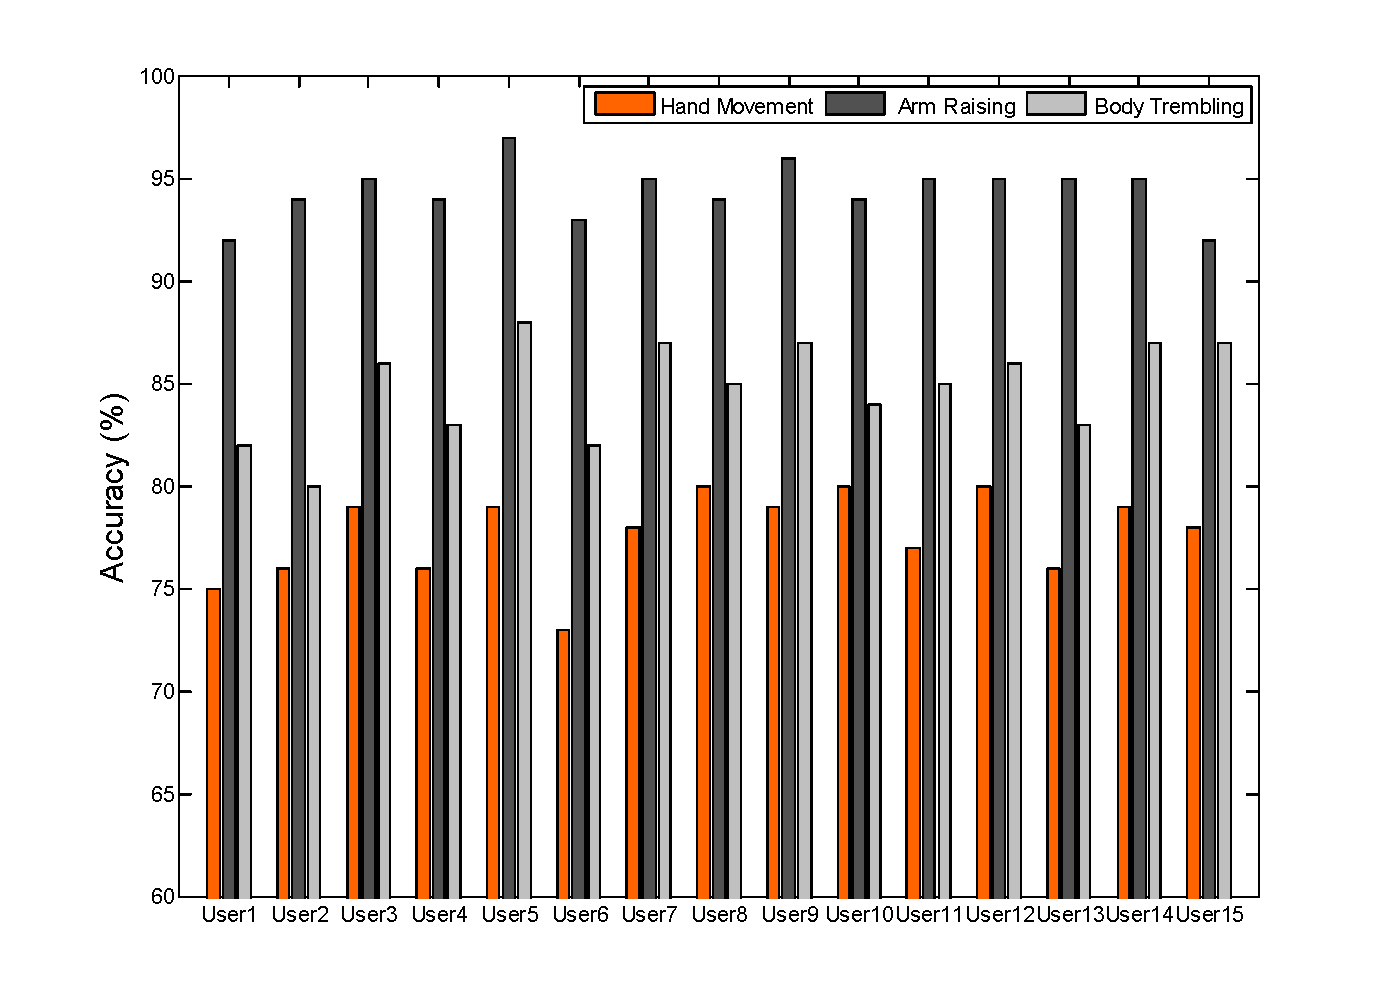
\includegraphics[width=0.52\linewidth]{Figures/micro_movement_zhu.pdf}
 \caption{Detection accuracy of micro body movement.}\label{fig:micro_movement_zhu}
\end{figure}

\begin{figure}
 \centering
   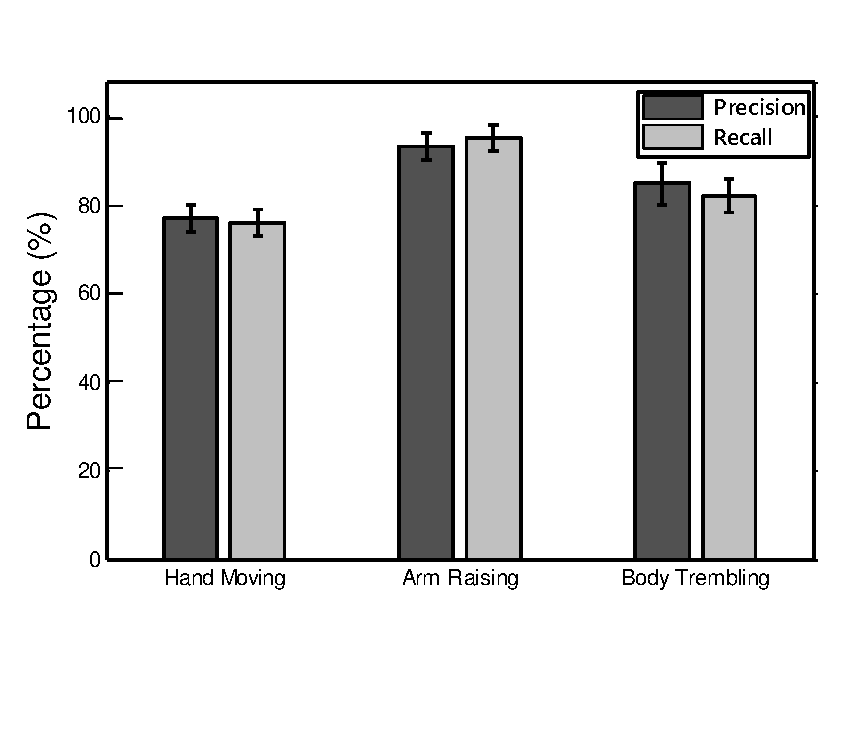
\includegraphics[width=0.52\linewidth]{Figures/micro_combine1.pdf}
 \caption{Micro body movement}\label{fig:micro_combine}
\end{figure}



 \subsubsection{Performance of acoustic events detection}
To study the detection accuracies of different acoustic events, we compare the groundtruth recorded by the camera with the detected results by our system. Table \ref{tab:sound} shows the results across 15 test participants. We can see that the accuracy for cough event is 88.9\%, which is relative lower with regard to other three events. The reason is that different user's cough pattern are different, the pre-defined parameters used in the system does not include all possible patterns. When we train the parameters of the detection algorithm, we only collect 120 sets of nighttime sound data. The data come from 40 (21 males and 19 females) volunteers of different ages (ages 15 to 60) who are prone to snoring, coughing, or somniloquy at night. So in order to further improve the detection accuracy, we can train particular parameters for more different users.

\begin{table}[!thbp]
 \tabcolsep1pt
  \centering  % ������
  \renewcommand\arraystretch{0.3}
  \caption{The confusion matrix of acoustic events detection.}\label{tab:sound}
\begin{tabular}{c| c | c | c | c | c | c}
   \hline
   &\multicolumn{1}{ c|}{ }
   & \multicolumn{4}{ c|}{ }\\
   \multirow{2}*{}
&\multicolumn{1}{c|}{\multirow{2}*{{ Result}}}
&\multicolumn{4}{c|}{{ Prediction}}
& \multirow{4}*{{ Recall}} \\
    %&\multicolumn{5}{ c |}{\textbf{\small Prediction}} \\
   % & \multicolumn{5}{ c |}{ } \\
    \cline{3-6}
    & & & & & \\
    \multicolumn{1}{c|}{{}}
    &  \multicolumn{1}{c|}{{}}
    &  \multicolumn{1}{c|}{{ Snore}}
    &  \multicolumn{1}{c|}{{ Cough}}
    &  \multicolumn{1}{c|}{{ Somniloquy}}
    &  \multicolumn{1}{c|}{{ Other}}   \\
    & & & & & \\
     \cline{1-7}
    & & & & & \\
    \multirow{5}{*}{\begin{sideways}{{ Groundtruth}}\end{sideways}}
    &   { Snore}   & {\bf{{96}}}    &   $0$      &   $0$      &   $9$    &   {91.4\%}\\
    & & & & & \\
    \cline{2-7}
    & & & & & \\
   &   { Cough}   &   $3$      &   {\bf{{64}}}     &   $0$      &   $4$   &   {90.1\%} \\
    & & & & & \\
     \cline{2-7}
    & & & & & \\
    &   { Somniloquy}   &   $0$      &   $3$      &  {\bf{{42}}}      &   $2$  &   {89.4\%}  \\
    & & & & & \\
     \cline{2-7}
    & & & & & \\
    &   { Other}   &   $0$      &   $5$      &   $4$      &   {\bf{{325}}}   &   {97.3\%} \\
    & & & & & \\
    \hline
    & & & & & \\
    &   { Precision}      &   {96.9\%}   &   {88.9\%}   &   {91.3\%}   &   {95.6\%}    \\
    & & & & & \\
    \hline
   \end{tabular}
\end{table}


\subsection{Overall performance}

\subsubsection{Performance of sleep stage detection}
In order to prove that the detected events not only reflect the user's sleep habits, but also effectively divide the sleep stage in order to assess the quality of sleep, we regard the reported results from Fitbit Charge2 as the ground truth.  \textcolor{blue}{We randomly selected 50 sets of nocturnal sleep data from 210 sets of sleep data collected from 15 participants for 2 weeks as the test data, what's more, we need to make sure that no less than 3 sets of nocturnal sleep data in these test data come from the same participant. It is worth mentioning that, {\ systemname} bases on the event detected by each submodule every 5 minutes to determine the sleep stage.} The average values of precision and recall are shown in Table \ref{tab:sleep stage}. From this table, we can see that although {\systemname} may often make misjudgement between light sleep stage and REM, the overall detection performance of {\systemname} is satisfying.

\begin{table}[!thbp]
	\tabcolsep1pt
	\centering  % ������
	\renewcommand\arraystretch{0.4}
	\caption{\textcolor{blue}{Performance of sleep stage detection.}}\label{tab:sleep stage}
	\begin{tabular}{c| c | c | c | c | c}
		\hline
		&\multicolumn{1}{ c|}{ }
		& \multicolumn{3}{ c|}{ }\\
		\multirow{2}*{}
		&\multicolumn{1}{c|}{\multirow{2}*{{ Result}}}
		&\multicolumn{3}{c|}{{ Prediction}}
		& \multirow{3}*{{ Recall}} \\
		%&\multicolumn{5}{ c |}{\textbf{\small Prediction}} \\
		% & \multicolumn{5}{ c |}{ } \\
		\cline{3-5}
		& & & & & \\
		\multicolumn{1}{c|}{{}}
		&  \multicolumn{1}{c|}{{}}
		&  \multicolumn{1}{c|}{{ REM}}
		&  \multicolumn{1}{c|}{{ Light Sleep}}
		&  \multicolumn{1}{c|}{{ Deep Sleep}} \\
		& & & & & \\
		\cline{1-6}
		& & & & & \\
		\multirow{4}{*}{\begin{sideways}{{ Groundtruth}}\end{sideways}}
		&   { REM}   & {\bf{{476}}}    &   $143$      &   $61$     &   {70.0\%}\\
		& & & & & \\
		& & & & & \\
		\cline{2-6}
		& & & & & \\
		&   { Light Sleep}   &   $131$      &   {\bf{{508}}}     &   $91$      &   {69.6\%} \\
		& & & & & \\
		\cline{2-6}
		& & & & & \\
		&   { Deep Sleep}   &   $63$      &   $113$      &  {\bf{{262}}}      &   {59.8\%}  \\
		& & & & & \\
		\cline{1-6}
		& & & & & \\
		&   { Precision}      &   {71.0\%}   &   {66.5\%}   &   {63.3\%}   \\
		& & & & & \\
		\hline
	\end{tabular}
\end{table}

\subsubsection{Evaluation on the effect of respiratory amplitude on sleep stage detection}
When we detect the hand's position in the abdomen or chest, we use the magnitude of the acceleration to estimate the amplitude of the respiration. To assess the effectiveness of {\systemname}'s detection of respiration amplitude, we evaluated the performance of the sleep stage test separately in two cases that with considering respiration amplitude and without considering respiration amplitude. And then we can measure the contributions of it for classification of the sleep stage, as we can see in Table \ref{tab:respiratory}. Obviously, When we consider the division of the sleep stage, combining breathing amplitude as a feature with other features, we find that the precision and recall of each sleep stage improve, which proves the effectiveness of our detection of respiration amplitude.

\begin{table} \footnotesize
	\centering  % ������
	\renewcommand\arraystretch{0.3}
	\caption{\textcolor{blue}{Evaluation of respiration amplitude contribution}}\label{tab:respiratory}
	\begin{tabular}{c| c | c | c | c | c | c| c |}
		\cline{2-8}
		&\multicolumn{1}{ c|}{ }
		&\multicolumn{2}{ c|}{ }
		&\multicolumn{2}{ c|}{ }
		& \multicolumn{2}{ c|}{ }\\
		%  \multirow{4}*{}
		&\multicolumn{1}{c|}{}
		&\multicolumn{2}{c|}{\textbf{\scriptsize REM}}
		&\multicolumn{2}{c|}{\textbf{\scriptsize Light Sleep}}
		&\multicolumn{2}{c|}{\textbf{\scriptsize Deep Sleep}} \\
		%&\multicolumn{5}{ c |}{\textbf{\small Prediction}} \\
		% & \multicolumn{5}{ c |}{ } \\
		\cline{2-8}
		& & & & & & &\\
		\multicolumn{1}{c|}{\textbf{}}
		&  \multicolumn{1}{c|}{\textbf{Features}}
		&  \multicolumn{1}{c|}{\scriptsize Precision}
		&  \multicolumn{1}{c|}{\scriptsize Recall}
		&  \multicolumn{1}{c|}{\scriptsize Precision}
		&  \multicolumn{1}{c|}{\scriptsize Recall}
		&  \multicolumn{1}{c|}{\scriptsize Precision}
		&  \multicolumn{1}{c|}{\scriptsize Recall}\\
		& & & & & & &\\
		\cline{2-8}
		& & & & & & &\\
		\multirow{5}{*}
		&   \textbf{\scriptsize Without Respiration Amplitude}   & $62.9\%$    &   $63.4\%$      &   $59.4\%$      &   $63.9\%$    &   $57.7\%$ &  $54.1\%$ \\
		& & & & & & &\\
		\cline{2-8}
		& & & & & & &\\
		&   \textbf{\scriptsize With Respiration Amplitude}   &   $71.0\%$      &   $70.0\%$     &   $66.5\%$      &   $69.7\%$   &   $63.3\%$ &   $59.8\%$ \\
		& & & & & & &\\
		
		\cline{2-8}
		
	\end{tabular}
\end{table}


\subsubsection{Performance comparison}
To our knowledge, in the current actigraphy-based work, there is no clear baseline for sleep stage detection performance for us. So we
decided to compare {\systemname} with the sleep detection app, Sleep As Android, that has been widely used in the marketplace, in addition,
we also considered a comparison with Sleep Hunter \cite{gu2016sleep}. Table \ref{tab:comparison} shows the performance of the sleep stage
detection, Sleep As Android can only detect light sleep stage and the deep sleep stage, so we only compared the performance of these two
stages.

 \begin{table} \footnotesize
	\centering  % ������
	\renewcommand\arraystretch{0.3}
	\caption{\textcolor{blue}{Performance Comparison}}\label{tab:comparison}
	\begin{tabular}{c| c | c | c | c | c |}
		\cline{2-6}
		&\multicolumn{1}{ c|}{ }
		&\multicolumn{2}{ c|}{ }
		&\multicolumn{2}{ c|}{ }\\
		%  \multirow{4}*{}
		&\multicolumn{1}{c|}{}
		&\multicolumn{2}{c|}{\textbf{\scriptsize Light Sleep}}
		&\multicolumn{2}{c|}{\textbf{\scriptsize Deep Sleep}} \\
		%&\multicolumn{5}{ c |}{\textbf{\small Prediction}} \\
		% & \multicolumn{5}{ c |}{ } \\
		\cline{2-6}
		\multicolumn{1}{c|}{\textbf{}}
		&  \multicolumn{1}{c|}{\diagbox{System}{Stage}}
		&  \multicolumn{1}{c|}{\scriptsize Precision}
		&  \multicolumn{1}{c|}{\scriptsize Recall}
		&  \multicolumn{1}{c|}{\scriptsize Precision}
		&  \multicolumn{1}{c|}{\scriptsize Recall}\\
		\cline{2-6}
		& & & & & \\
		\multirow{5}{*}
		&   \textbf{\scriptsize SleepGuard}   & $66.5\%$    &   $69.6\%$      &   $63.3\%$      &   $59.8$  \\
		& & & & &  \\
		\cline{2-6}
		& & & & & \\
		&   \textbf{\scriptsize Sleep As Android}   &   $27.8\%$      &   $35.4\%$     &   $35.7\%$      &   $50.2\%$   \\
		\cline{2-6}
		& & & & & \\   
		&   \textbf{\scriptsize Sleep Hunter}   &   $66.74\%$      &   $66.11\%$     &   $60.00\%$      &   $50.73\%$   \\
		
		\cline{2-6}
		
	\end{tabular}
\end{table}


As we can see, {\systemname} can not only perform better on sleep stage detection than Sleep As Android, but also detect one more sleep stage. \textcolor{blue}{As for Sleep Hunter, our system's detection ability is slightly better than its. This may be because {\systemname} detects sleep-related events with better performance and incorporates respiratory amplitude considerations. And our system can provide richer sleep data for users and take more factors that affect sleep quality into consideration, making users understand their sleep more easily and improve their sleep quality more effectively.} Further, we show our superior in function comapared with other similar sleep detection products, including Sleep As Android, Sleep Hunter, sleepMonitor \cite{sleepmonitor}, Sleeptracker \cite{sleeptracker}, Fitbit, isleep \cite{hao2013isleep}, Jawbone \cite{Jawbone},ubiSleep \cite{pombo2016ubisleep}, in Table \ref{tab:function}. As we have shown, {\systemname} can detect a wider range of sleep events to provide a better user experience.

\begin{table*}\scriptsize
\setlength{\abovecaptionskip}{0.8pt}
  \centering  % ������
  \tabcolsep10pt
  \arrayrulewidth1pt
  \caption{Systems for support sleep}\label{tab:function}
  \renewcommand{\multirowsetup}{\centering}
  \noindent\makebox[\textwidth]{%
        \begin{tabularx}{1.0\textwidth}{|c|c|c|c|c|c|c|}
        \cline{1-7}
        \multicolumn{1}{|c|}{\multirow{2}*{\textbf{\scriptsize System}}}
        &\multicolumn{6}{c|}{\textbf{ \scriptsize Detected Events}} \\
         \cline{2-7}
    &  \multicolumn{1}{c|}{\textbf{ \scriptsize Heart Rate }}
    &  \multicolumn{1}{c|}{\textbf{ \scriptsize Acoustic Event }}
    &  \multicolumn{1}{c|}{\textbf{ \scriptsize Sleep Posture }}
     &  \multicolumn{1}{c|}{\textbf{ \scriptsize body Movement }}
      &  \multicolumn{1}{c|}{\textbf{ \scriptsize hand position}}
       &  \multicolumn{1}{c|}{\textbf{ \scriptsize Sleep Stage}} \\
        \cline{1-7}
        \multirow{7}{2cm}
        {\textbf{SleepGuard\\Sleep as Android\\Sleep Hunter\\SleepMonitor\\Sleeptracker\\isleep \\Fitbit\\Jawbone\\ ubiSleep } }
        & &$\checkmark$ & $\checkmark$ &  $\checkmark$  &$\checkmark$ &$\checkmark$\\
        & &$\checkmark$ & & & &$\checkmark$\\
        & & $\checkmark$& &$\checkmark$ & &$\checkmark$\\
        & & & $\checkmark$ & & &\\
        &$\checkmark$ & & & & &$\checkmark$\\
         & &$\checkmark$ &   &$\checkmark$ & &\\
         &$\checkmark$ & & & & &$\checkmark$ \\
        & & & & & &$\checkmark$ \\
        & $\checkmark$&$\checkmark$ & & & &\\
        \cline{1-7}
 \end{tabularx}}
\end{table*}

\subsubsection{User survey}
In order to evaluate whether {\systemname} can provide help in the assessment of sleep quality and has a good user experience, we conducted a user survey of 15 volunteers participating in our experiments. In our survey, we asked participants to fill out our questionnaire based on PSQI \cite{carpenter1998psychometric} every morning during the experiment, in order to get their subjective feeling of sleep quality and use experience for our system. We use the following questions in our survey, which includes:
\begin{enumerate}
  \item Subjective sleep quality (5 levels, 1 for excellent and 5 for worst)
  \item Sleep duration
  \item Sleep disturbances
  \item Daytime dysfunction
\end{enumerate}

\textcolor{blue}{The average 14-day sleep quality score for 15 individuals are shown in Table. \ref{tab:quality}, we have listed three kinds of sleep quality assessment mechanims, namely, {\systemname}, Fitbit and user survey, where the sleep quality score obtained by user survey comes from the comprehensive scores of the questionnaires based on the above aspects. For the above four items, each one is rated on a 1-5 scale. These component scores are then summed to yield a score, which has a range of 0-20. And we divide each five scores into one and eventually divide the total score into four levels, recorded as 0-3, representing poor, general, good and excellent respectively, that is higher scores indicate better sleep quality. From the table, we can see the result is satisfactory and representative to some extent.} In addition, we also ask whether users are interested in these events, such as sleep posture, hand position, which detected by {\systemname}. 80\% of participants believe that the detection of sleep posture is very necessary, showing their sleep posture can not only help people to avoid health problems caused by long-term improper sleeping posture, but also help us find out the reasons for the next day's physical discomfort, such as dizziness, muscle soreness may be due to improper sleeping position. 60\% of the participants thought it useful to detect their hand position in the supine position and even one user mentioned that he did often have nightmares and that he found his hands were often placed on his chest. And {\systemname} was able to remind him to avoid such a hand position when sleeping. However, only 20\% of them think it is necessary to calculate the number of body rollover, but the detection of body rollover is very useful in the division of sleep stage.


\begin{table} \footnotesize
  \centering  % ������
  \renewcommand\arraystretch{0.3}
  \caption{\textcolor{blue}{Results of sleep quality assessment}}\label{tab:quality}
\begin{tabular}{c| c | c | c | c | c |c |c |c |c |c| c |c |c |c |c |c |c|}
   %\cline{2-6}
   %&\multicolumn{1}{ c|}{ }
   %&\multicolumn{2}{ c|}{ }
  % &\multicolumn{2}{ c|}{ }\
    %&\multicolumn{1}{c|}{}
   %&\multicolumn{2}{c|}{\textbf{\scriptsize Light Sleep}}
  % &\multicolumn{2}{c|}{\textbf{\scriptsize Deep Sleep}} \\
    %&\multicolumn{5}{ c |}{\textbf{\small Prediction}} \\
   % & \multicolumn{5}{ c |}{ } \\
    \cline{2-17}
    \multicolumn{1}{c|}{\textbf{}}
    &  \multicolumn{1}{c|}{\diagbox{System}{User}}
    &  \multicolumn{1}{c|}{\scriptsize User 1}
    &  \multicolumn{1}{c|}{\scriptsize User 2}
    &  \multicolumn{1}{c|}{\scriptsize User 3}
    &  \multicolumn{1}{c|}{\scriptsize User 4}
    &  \multicolumn{1}{c|}{\scriptsize User 5}
    &  \multicolumn{1}{c|}{\scriptsize User 6}
    &  \multicolumn{1}{c|}{\scriptsize User 7}
    &  \multicolumn{1}{c|}{\scriptsize User 8}
    &  \multicolumn{1}{c|}{\scriptsize User 9}
    &  \multicolumn{1}{c|}{\scriptsize User 10}
    &  \multicolumn{1}{c|}{\scriptsize User 11}
    &  \multicolumn{1}{c|}{\scriptsize User 12}
    &  \multicolumn{1}{c|}{\scriptsize User 13}
    &  \multicolumn{1}{c|}{\scriptsize User 14}
    &  \multicolumn{1}{c|}{\scriptsize User 15}\\
     \cline{2-17}
    & & & & & & & & & & & & & & & & \\
    \multirow{16}{*}
    &   \textbf{\scriptsize SleepGuard}  & $3$ & $3$ & $0$ & $2$ & $2$ & $1$ & $3$ & $0$ & $2$ & $2$ & $2$ & $2$ & $1$ & $0$ & $2$ \\
   & & & & & & & & & & & & & & & &\\
    \cline{2-17}
   & & & & & & & & & & & & & & & &\\
   &   \textbf{\scriptsize Fitbit}   & $3$ & $3$ & $0$ & $3$ & $1$ & $0$ & $2$ & $3$ & $2$ & $2$ & $2$ & $2$ & $2$ & $1$ & $2$\\
    \cline{2-17}
    & & & & & & & & & & & & & & & & \\
    &   \textbf{\scriptsize User survey}  & $3$ & $2$ & $0$ & $2$ & $2$ & $0$ & $3$ & $1$ & $1$ & $2$ & $2$ & $3$ & $0$ & $0$ & $2$ &  \\
   \cline{2-17}

   \end{tabular}
\end{table}

%\begin{figure}
 %\centering
% 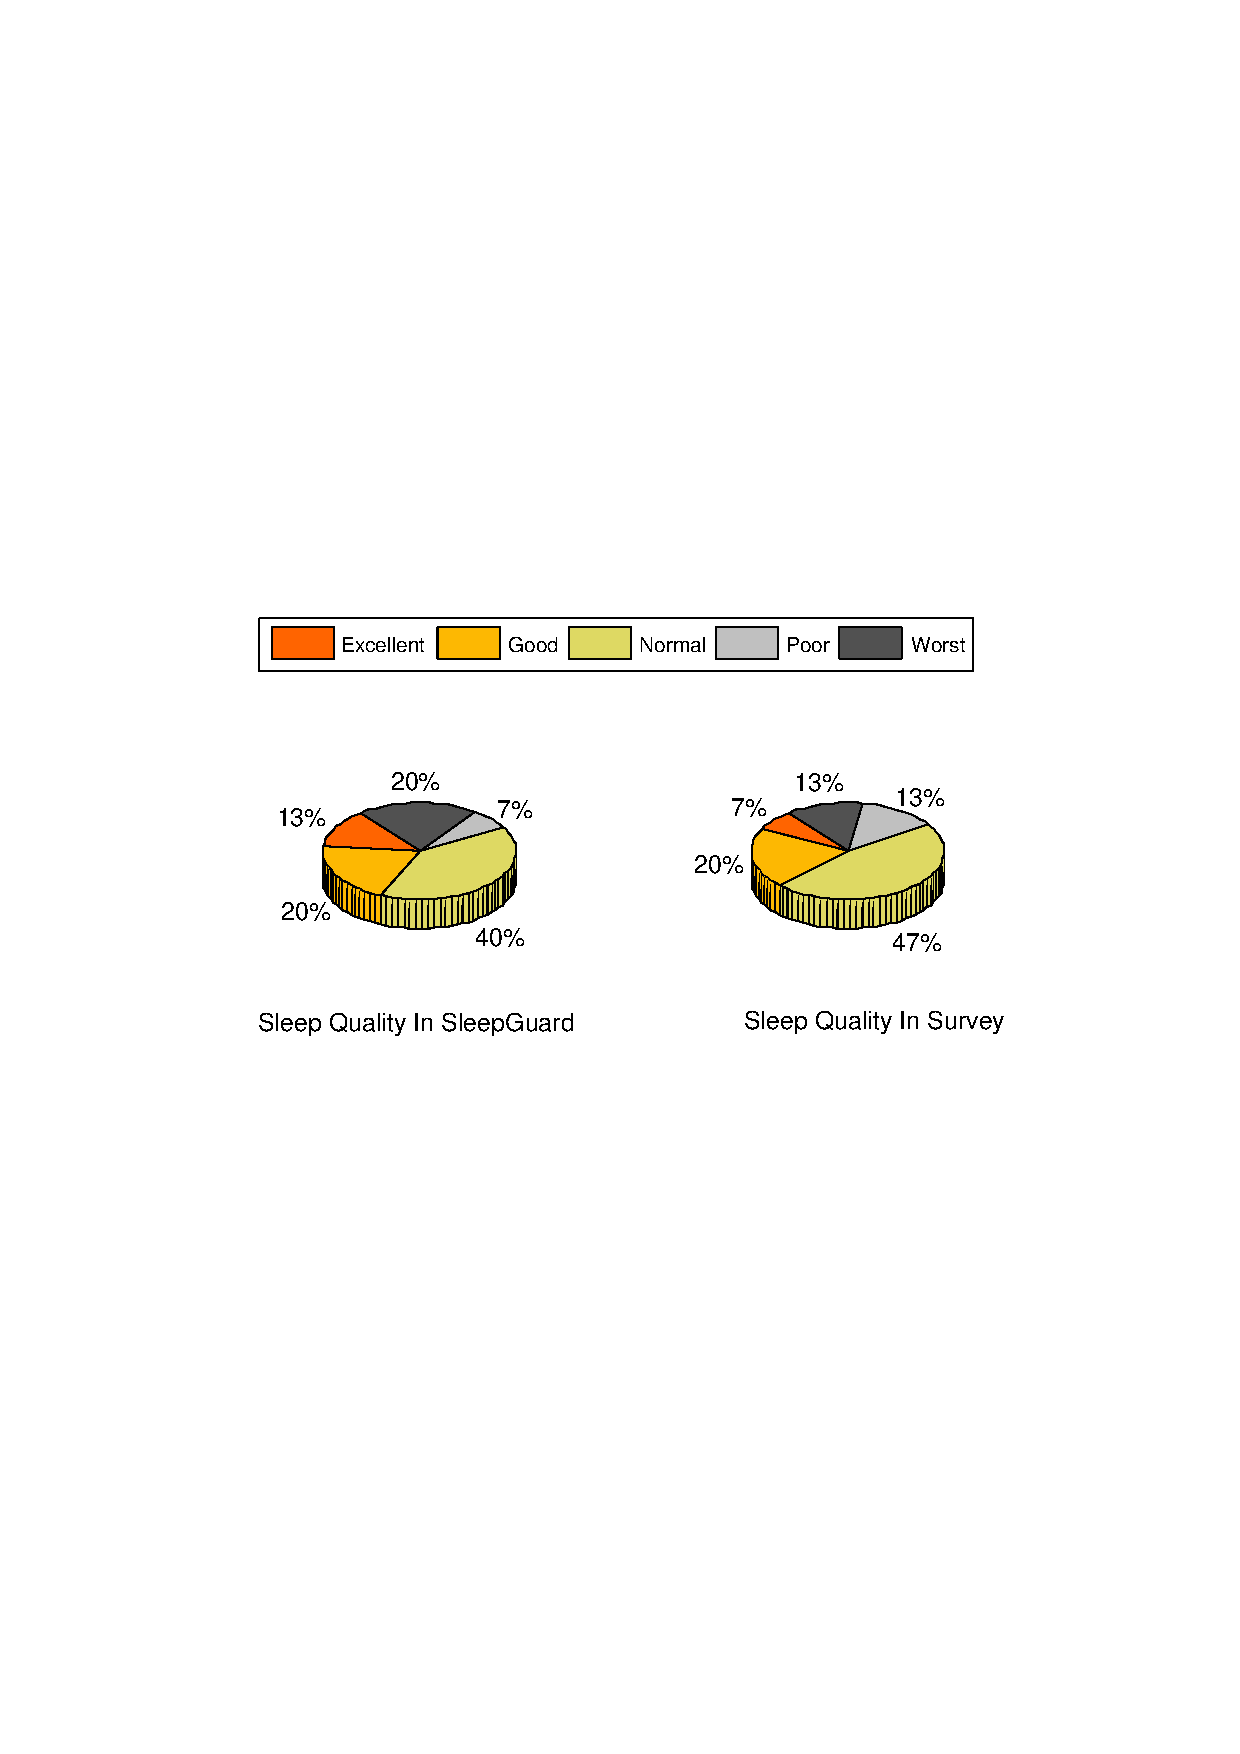
\includegraphics[width=0.52\linewidth]{Figures/quality.pdf}
 %\caption{Participants' sleep quality distribution}\label{fig:quality}
%\end{figure}
